\section{Specifications}
\label{sec:specifications}
This chapter lays out the specification used to design the wavelength division modulation (WDM) system.

\begin{itemize}
 \item The inputs and outputs of the system are optical.
 \item The signals will not be converted to the electrical domain at any stage (no O/E/O). 
 \item Single mode fibre will be used.
 \item 4 channels are used.
 \item TX and RX signals use a common fiber.
 \item The system can perform both MUX and DEMUX operations.
 \item The channel wavelengths are spaced \qty{20}{\nm} apart.
\end{itemize}

The inputs and outputs of the system are all optical, as transponders fall outside the 
scope of the system. By also keeping the signals in the optical domain, the mux and demux 
operation has to be performed in the optical domain. Single mode fiber will be used, 
meaning it is up to the user to make sure that each input is matched to the correct channel. 
Single mode fiber was chosen such that modal dispersion doesn't have to be accounted for. 
Lastly, individual channels will be spaced \qty{20}{\nm} apart, making it a CWDM system.

From the above requirements a MUX/DEMUX system will be designed. An overiew of the of these 
systems in a link is given in figure \ref{fig:link_overview} below.

\begin{figure}[ht]
    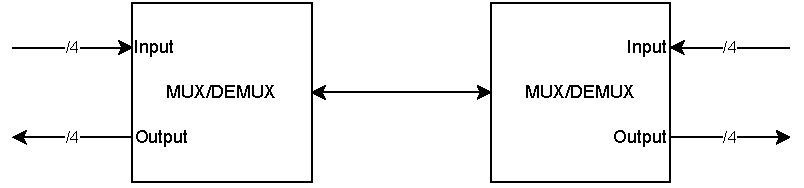
\includegraphics[width=\linewidth]{images/link_overview.pdf}
    \caption{Overview of MUX/DEMUX link}
    \label{fig:link_overview}
\end{figure}